\section{Evietania Charis Sujadi (1174051)}
\subsection{Pengertian}
adalah suatu sistem informasi yang berbasis komputer, dirancang untuk bekerja dengan menggunakan data yang memiliki informasi spasial . Sistem ini mengcapture, mengecek, mengintegrasikan, memanipulasi, menganalisa, dan menampilkan data yang secara spasial mereferensikan kepada kondisi bumi. \hfill\break
Aktifitas yang terjadi di bumi merupakan bagian dari ilmu Geografi.\hfill\break
\subsection{Sejarah}
pada 35000 tahun yang lalu, pada dinding gua Lascaux, Perancis, para pemburu Cro-Magnon menggambar hewan mangsa mereka, juga garis yang dipercaya sebagai rute migrasi hewan-hewan tersebut. pada catatan awal ini sejalan dengan dua elemen struktur pada sistem informasi gegrafis modern sekarang ini, arsip grafis yang terhubung ke database atribut.\hfill\break
Pada tahun 1700an sebuah teknik survey modern untuk pemetaan topografis diterapkan, termasuk versi awal pemetaan tematis, misalnya untuk keilmuan atau data sensus.\hfill\break
pada awal abad ke 20 memperlihatkan pengembangan “litografi foto” dimana peta dipisahkan menjadi beberapa lapisan . Perkembangan perangkat keras komputer yang dipacu oleh penelitian senjata nuklir membawa aplikasi pemetaan menjadi multifungsi pada awal tahun 1960an.\hfill\break
Pada tahub 1967 merupakan awal pengembangan SIG yang bisa diterapkan di Ottawa, Ontario oleh Departemen Energi, Pertambangan dan Sumber Daya. dikembangkan oleh roger dimana, kemudian disebut CGIS (Canadian GIS – SIG Kanada), digunakan untuk menyimpan, menganalisis dan mengolah data yang dikumpulkan untuk Inventarisasi Tanah Kanada (CLI) sebuah inisiatif untuk mengetahui kemampuan lahan di wilayah pedesaan Kanada dengan memetakaan berbagai informasi pada tanah, pertanian, pariwisata, alam bebas, unggas dan penggunaan tanah pada skala 1:250000.\hfill\break
CGIS bertahan sampai tahun 1970-an dan memakan waktu lama untuk penyempurnaan setelah pengembangan, dan tidak bisa bersaing denga aplikasi pemetaan komersil yang dikeluarkan beberapa vendor seperti Intergraph. Perkembangan perangkat keras mikro komputer memacu vendor lain seperti ESRI dan CARIS berhasil membuat banyak fitur SIG, menggabung pendekatan generasi pertama pada pemisahan informasi spasial dan atributnya, dengan pendekatan generasi kedua pada organisasi data atribut menjadi struktur database. Perkembangan industri pada tahun 1980 dan 1990 memacu sebuah pertumbuhan SIG pada workstation UNIX dan komputer pribadi. Pada akhir abad ke 20, pertumbuhan yang cepat di berbagai sistem dikonsolidasikan dan distandarisasikan menjadi platform lebih sedikit, dan para pengguna mulai mengekspor menampilkan data SIG lewat internet, yang membutuhkan standar pada format data dan transfer
\subsection{Koordinat}
Koordinat didapatkan dari hasil perpotongan antara garis latitude (Y) / lintang dan garis longitude(X) / garis bujur sehingga bisa menunjukan suatu lokasi pada suatu daerah.
\subsection{Data Geospasial}
Data yang aspek fisiknya dan administratif dari sebuah objek geografis. Aspek fisik di sini mencakup pula bentuk anthropogenic dan bentuk alam baik yang terdapat di permukaan maupun di bawah permukaan bumi. 
\subsection{Link}
\href{https://youtu.be/eby2SXgrvbU}{Pencet Aku}
\subsection{Plagiarism}
\begin{figure}[H]
	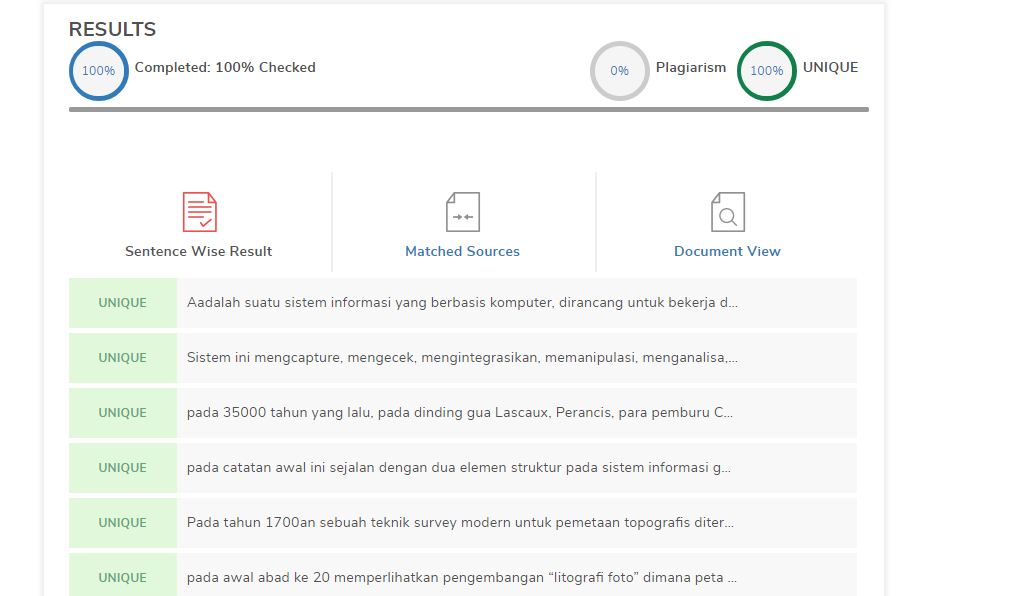
\includegraphics[width=4cm]{figures/1174051/1/1.png}
	\centering
	\caption{Bukti Tidak Melakukan Plagiat}
\end{figure}

\subsubsection{List}
\begin{enumerate}
	\item Satu
	\item Dua
\end{enumerate}

\begin{itemize}
	\item Satu
	\item Dua
\end{itemize}

\href{link kamu}{alias}
contoh link
\href{https://www.google.com/}{klik me}